\chapter{Definition 'gesunder Lebensstil'}
\authortoc{\bastian}{\chapterident}
Definition des WHO: “Die Gesundheit ist ein Zustand des vollständigen körperlichen, geistigen und sozialen Wohlergehens und nicht nur das Fehlen von Krankheit oder Gebrechen.” \cite{gesundheit_definition}.
\newline
Einen gesunden Lebensstil beinhaltet nicht nur die Ernährung, sondern deckt auch einige andere Themenkreise ab, welche ansonsten nicht so oft thematisiert werden. Dazu haben wir einige Themen herausgesucht, welche unserer Meinung nach die Wichtigsten sind, um gesund zu leben. Diese Themen wären: Ernährung, Bewegung, Schlaf, Zeitmanagement und diverse Gewohnheiten. Auf diese werden wir nun im Detail eingehen.
\section{Ernährung}
\authortoc{\dario}{\sectionident}
Die Ernährung ist die Aufnahme von Nahrungsmittel, welche unserem Körper die notwendige Energie zur Verfügung stellt. Somit spielt die Ernährung eine wichtige Rolle bei einem gesunden Lebensstil. Wenn man nicht auf die Ernährung achtet, zum Beispiel zu viel Fette oder zu wenig Vitamine zu sich nimmt, kann dies schlimme Folgen haben. Dies kann zu Herz- Kreislaufstörungen, Über- /Untergewicht, Diabetes Typ 2 und vielem mehr führen.
\newline
Für die Definition, was eine gesunde Ernährung bedeutet, beziehen wir uns auf die Schweizer Ernährungspyramide.
\newline
\begin{figure}[!ht]
  \centering
  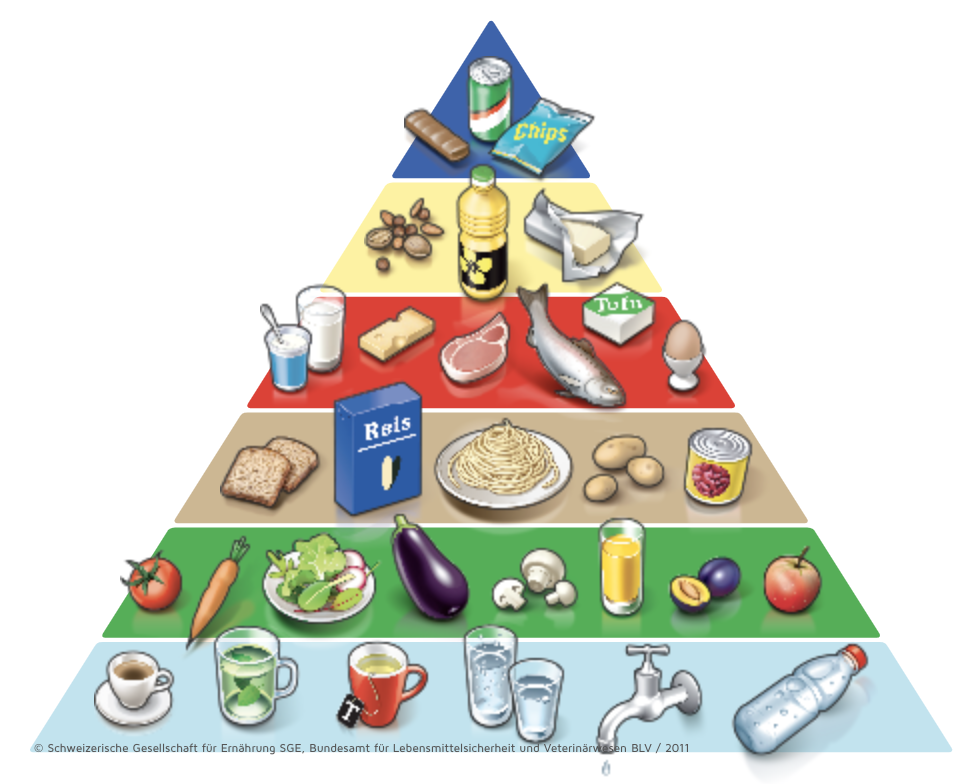
\includegraphics[width=0.5\linewidth]{./images/lebensmittelpyramide.png}
  \caption{Die schweizerische Lebensmittelpyramide}
  \label{fig:pyramide}
  \captionsetup{font={footnotesize}}
  \caption*{\url{https://www.sge-ssn.ch/ich-und-du/essen-und-trinken/ausgewogen/schweizer-lebensmittelpyramide/}}
\end{figure}
\pagebreak
Diese Ernährungspyramide besteht aus sechs Stufen:
\begin{enumerate}
  \item \textbf{Getränke} - Es wird empfohlen, ein bis zwei Liter Flüssigkeit pro Tag zu sich zu nehmen. Diese Getränke sollten am Besten ungesüsst sein. Mögliche Getränke wären zum Beispiel Wasser, Tee oder Kaffee. \cite{stufe_getraenke}
  \item \textbf{Gemüse und Früchte} - Es wird empfohlen, drei Portionen Gemüse und zwei Portionen Früchte pro Tag zu essen. Dabei entspricht eine Portion ca. 120 g.
  \newline
  Mit dieser Stufe nimmt man wichtige Vitamine, Mineralstoffe und Nahrungsfasern auf.
  \newline
  Die Auswahl an Früchten und Gemüse sollte abwechslungsreich sein, um ein möglichst breites Spektrum an Vitaminen, Mineralstoffen usw. abzudecken. \cite{stufe_gemuese_fruechte}
  \item \textbf{Getreideprodukte, Kartoffeln und Hülsenfrüchte} - Es wird empfohlen, täglich drei Portionen aus dieser Stufe zu konsumieren. Die Grösse der Portionen ist nahrungsmittelabhängig. Zum Beispiel 180 g bis 300 g Kartoffeln oder 75 g bis 125 g Brot.
  \newline
  Mit dieser Stufe nimmt man hauptsächlich Kalorien auf, die wichtige Energie für Muskeln, Gehirn und vielem mehr liefert. \cite{stufe_getreideprodukte_kartoffeln_huelsenfruechte}
  \item \textbf{Milchprodukte, Fleisch, Fisch, Eier und Tofu} - Diese Stufe wurde in zwei Gruppen unterteilt: 
    \begin{enumerate}
    \item \textbf{Milchprodukte} - Es wird empfohlen, täglich drei Portionen Milch und Milchprodukte zu konsumieren. Die Grösse der Portionen ist auch wieder nahrungsmittelabhängig. Zum Beispiel 2 dl Milch oder 150 g bis 200 g Joghurt, Quark usw.
    \newline
    Mit diesen Nahrungsmitteln nehmen wir Proteine und Kalzium auf. Diese Stoffe sind wichtig für unsere Muskeln, Immunsystem, Knochen und vieles mehr. \cite{stufe_milch_milchprodukte}
    \item \textbf{Fleisch, Fisch Eier und Tofu} - Es wird empfohlen, täglich eine Portion Fleisch, Fisch, Eier oder Tofu zu konsumieren. Die Grösse der Portion ist auch wieder Nahrungsmittel abhängig. Zum Beispiel 2 - 3 Eier oder 100 g bis 120 g Fleisch.
    \newline
    Mit den drei Portionen Milchprodukten ist der tägliche Proteinbedarf noch nicht gedeckt.
    \newline
    Daher wird zusätzlich eine Portion proteinreiches Lebensmittel empfohlen. Diese kann jedoch auch mit einer vierten Portion Milchprodukte umgangen werden. \cite{stufe_fleisch_fisch_eier_tofu_2}
  \end{enumerate}
  \item \textbf{Öle, Fette und Nüsse} - Es wird empfohlen, täglich 20 g bis 30 g Pflanzenöl zu konsumieren. Davon sollte die hälfte Rapsöl sein. Pro Tag sollte zusätzlich 20 g bis 30 g ungesalzene Nüsse, Samen oder Kerne konsumiert werden.
  \newline
  Butter, Margarine, Rahm etc sollte nur sparsam verwendet werden.
  \newline
  Diese Stufe liefert viele Kalorien, lebensnotwendige Fettsäuren und fettlösliche Vitamine. \cite{stufe_le_fette_nuesse}
  \item \textbf{Süsses, Salziges und Alkoholisches} - Aus Ernährungssicht ist diese Stufe nicht notwendig. Jedoch für einen gesunden Lebensstil durchaus berechtigt. 
  Täglich sollte nur eine kleine Portion Lebensmittel aus dieser Stufe konsumiert werden.
  Auch Light- und Zero-Softgetränke zählen zu dieser Stufe. Sie beinhalten zwar wenig Kalorien, jedoch gewöhnt man sich dadurch an den süssen Geschmack und die Säuren machen die Zähne kaputt. \cite{stufe_suesses_salziges_alkoholisches}
\end{enumerate}
Die Übertragung der Ernährungspyramide auf eine Mahlzeit kann man mit der nächsten Grafik einfach veranschaulichen.
\newline
\begin{figure}[!hbpt]
  \centering
  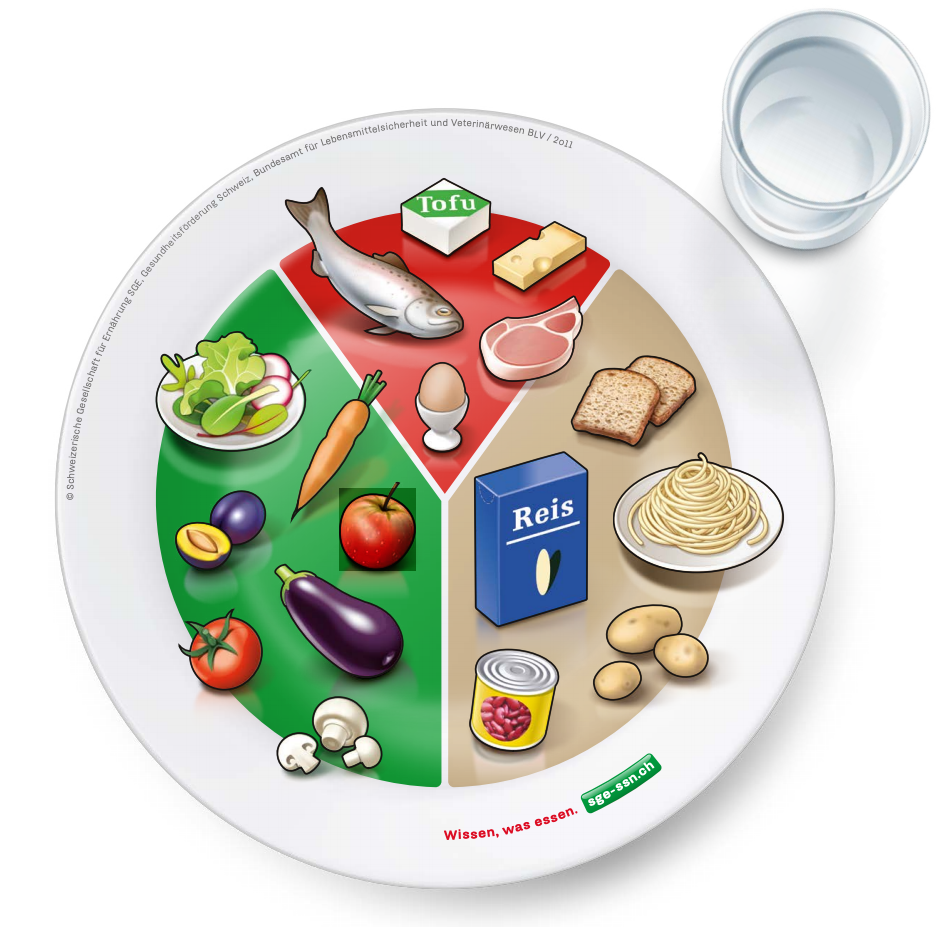
\includegraphics[width=0.5\linewidth]{./images/der_perfekte_teller.png}
  \caption{Optimaler Teller}
  \label{fig:teller}
  \captionsetup{font={footnotesize}}
  \caption*{\url{https://www.sge-ssn.ch/media/Merkblatt_der_optimale_Teller.pdf}}
\end{figure}
\newline
Fast die Hälfte des Tellers sollte aus Gemüse und Früchte bestehen. Ein kleiner Teil sollte aus Milchprodukte, Fleisch, Fisch oder Tofu bestehen. Der Rest des Tellers sollten Getreideprodukte, Kartoffeln oder Hülsenfrüchte sein. Dazu sollte man Wasser trinken.
\newline
Diese Zusammensetzung muss jedoch nicht für jede Person stimmen. Menschen, welche sich im Alltag wenig bewegen, verbrauchen weniger Energie. Für diese Personen kann man den optimalen Teller folgendermassen anpassen:
\newline
\begin{figure}[!hbpt]
  \centering
  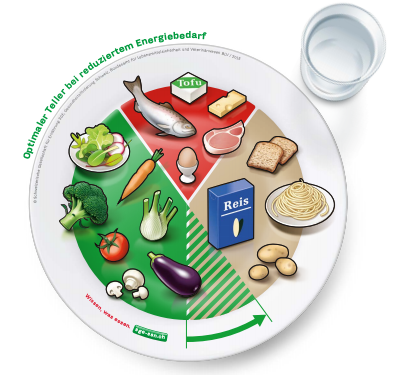
\includegraphics[width=0.5\linewidth]{./images/optimale_teller_energie.png}
  \caption{Optimaler Teller mit reduziertem Energiebedarf}
  \label{fig:teller_2}
  \captionsetup{font={footnotesize}}
  \caption*{\url{https://www.sge-ssn.ch/media/Merkblatt_der_optimale_Teller.pdf}}
\end{figure}
\newline
Dabei würde der Gemüse- und Früchte-Teil die Hälfte des Tellers einnehmen. Dafür nimmt man weniger Getreideprodukte, Kartoffeln oder Hülsenfrüchte zu sich.
\section{Bewegung}
\authortoc{\bastian}{\sectionident}
Das BAG macht darauf aufmerksam, dass jede körperliche Aktivität sehr gut für die Leistungsfähigkeit und die Gesundheit ist. Bewegung in regelmässigen Abständen ist sehr wichtig, um das Risiko für weitverbreitete Beschwerden und Krankheiten wie z. B. Übergewicht, Bluthochdruck, Herz-Kreislauferkrankungen und Diabetes 2 zu reduzieren.
\newline
Wer sich viel bewegt, lebt länger. Die Definition von Bewegung ist laut BAG “Jede Form der Bewegung, die eine Anspannung der Muskeln erfordert und den Energieverbrauch im Vergleich zum Ruhezustand erhöht”.
\newline
Ebenfalls verbessert die Bewegung die Lebensqualität, indem sie sich positiv auf das psychische Wohlbefinden auswirkt. Dies hängt mit Hormonen zusammen. Laut der CSS-Versicherung, lässt jede Art von Bewegung im Gehirn gewisse Hormone ausschütten, welche alle eine andere Auswirkung auf den Menschen haben \cite{hormone-bei-bewegung}. Es gibt zum einen die Ausschüttung von Stresshormonen, zum anderen schüttet der Körper auch Glückshormone aus. Bei den Stresshormonen spielen Cortisol sowie Adrenalin und Noradrenalin eine Rolle, damit der Körper genug Energie zugeführt bekommt. Bei den Glückshormonen geht man davon aus, dass Dopamin sowie Serotonin einen Glückszustand auslösen und dabei das empfinden von Schmerzen herabstufen.
\newline
\begin{figure}[!ht]
  \centering
  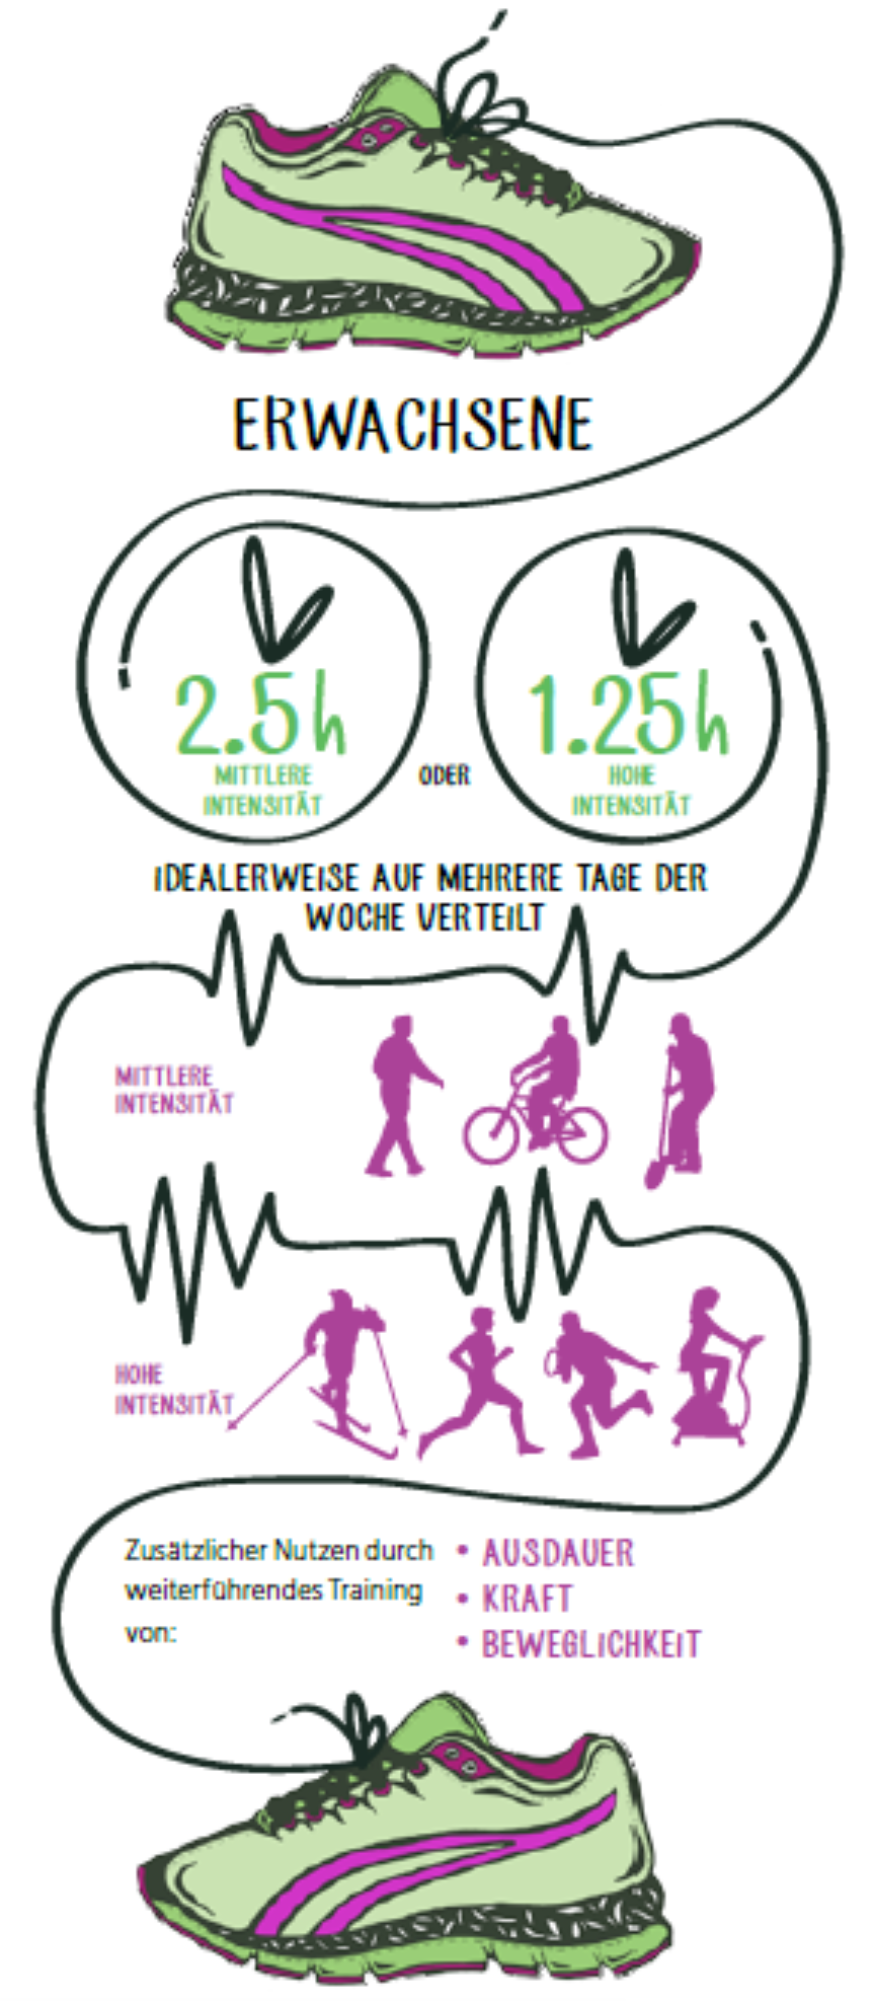
\includegraphics[width=0.38\linewidth]{./images/bewegungsempfehlungen-ew-dt.png}
  \caption{Grafik vom BAG zur Bewegungsempfehlung von Erwachsenen Menschen.}
  \label{fig:bewegungsempfehlungen}
  \captionsetup{font={footnotesize}}
  \caption*{\url{https://www.bag.admin.ch/bag/de/home/gesund-leben/gesundheitsfoerderung-und-praevention/bewegungsfoerderung/bewegungsempfehlungen.html}}
\end{figure}
\newline
Das BAG empfehlt für jeden Erwachsenen idealerweise mindestens 2 Stunden und 30 Minuten Bewegung pro Woche in Form von Alltagsaktivitäten oder Sport mit mittlerer Intensität \cite{bewegungsfoerderung}. Dazu gehört zum Beispiel das Fahrradfahren, das Gehen oder die Gartenarbeit. Diese Empfehlung kann auch durch Sport mit hoher Intensität ersetzt werden. Dabei wird mindestens 1h und 15 min Bewegung pro Woche als Basiswert genommen. Sportarten mit hoher Intensität sind zum Beispiel Rennen, Krafttraining, Skifahren und noch diverse andere. 
\section{Schlaf}
\authortoc{\bastian}{\sectionident}
“Der Schlaf ist eine grundlegende biologische Funktion und für das Wohlbefinden eines Menschen notwendig” so lautet die Definition vom Bundesamt für Statistik \cite{bundesamtfrstatistik_2015_schlafstoerungen}.
\newline
Der Schlaf sorgt für eine gute Lebensqualität, indem er sämtliche Kräfte wiederherstellt. Laut Gesundheit.de ist Schlaf auch bei Weitem keine passive Tätigkeit. Der Körper reagiert schwächer, jedoch finden wichtige Auf- und Abbauprozesse statt. Für einen gesunden Lebensstil sind zwei Phasen des Schlafs sehr wichtig. Dazu gehören die Tiefschlafphase sowie die Traumphase. In der Tiefschlafphase erholt sich der Körper und “repariert” unsere Organe. Die Traumphase ist wichtig für die psychische Erholung. Es gibt einige Menschen in der Schweiz, welche an Schlafstörungen leiden. Laut dem BFS leidet ein Viertel der Bevölkerung an Schlafstörungen. Diese haben zur Folge, dass man physische und psychische Gesundheitsprobleme erhalten kann oder das Diabetes sowie Adipositas Risiko steigt. Einen Mangel an Schlaf stört ebenfalls das Gedächtnis \cite{schlaf-grundbeduerfnis-und-lebenselixier}. Während des Schlafs werden Gelerntes und Erfahrungen verarbeitet und zugeordnet. Bei ständigem Mangel ist die Funktion des Gehirns eingeschränkt, sodass es nicht alles richtig verarbeiten kann. Der Schlaf hat weitere starke Einflüsse. Zum einen stärkt er das Immunsystem und zum anderen reguliert er den Hunger. Wenn man zu wenig schläft, ist man somit angreifbarer für diverse Infektionen. Ebenfalls wird das Gleichgewicht zwischen den Hormonen für Hunger stark gestört, was zu einem erhöhten Appetit führen kann.
\section{Zeitmanagement}
\authortoc{\jonas}{\sectionident}
Das Zeitmanagement wird von sehr vielen Menschen zu sehr unterschätzt. Viele Leben einfach von Tag zu Tag und lassen sich überraschen. Je mehr jedoch im Leben vorgeht, desto mehr geht vergessen, was vermeidbaren Stress entstehen lässt. 
\newline
Es empfehlt sich deshalb sehr, zumindest einen Monats- und/oder Wochenplan zu erstellen, welchen man mit einer ToDo Liste verbinden kann. So kann schon viel Stress vermeidet werden, da man eine Übersicht über die kommende Woche und das Unerledigte hat. 
\newline
Laut den Zahlen vom Bundesamt für Statistik von 2017 steigt die Anzahl der unter Stress leidenden immer mehr. 2012 gaben 18 \% der Befragten an, im Beruf aktiv unter Stress zu leiden. In der letzten Publikation von 2017 stieg dieser Wert auf 21 \% an \cite{bundesamtfrstatistik_2019_arbeitsbedingungen}. Ist eine Person über einen längeren Zeitraum Stress ausgesetzt, so kann sich das schlecht auf die mentale und physische Gesundheit auswirken \cite{stress-symptoms}. Auf den Körper bezogen kann es zu Kopfschmerzen, Schlafproblemen, einem hohen Blutdruck und unter anderem zu einem schwächeren Immunsystem führen. Mental kommt es meist zu Ängsten, Wut, Gefühlen von Überlastung, schwankende Laune, Konzentrationsproblemen, schlechtem Selbstbild und kann eine Depression verursachen. Auch das Verhalten einer Person kann sich anpassen. Symptome beim Verhalten sind Über- oder Unterernährung, Wutausbrüche, Probleme in Beziehungen und dem Vermeiden von Personen. Zudem greifen Personen, welche einen längeren Zeitraum unter Stress leiden, ofters zu Suchtmitteln wie Alkohol, Nikotin oder andere Drogen als Personen, welche verminderten oder gar keinen Stress haben.
\section{Gewohnheiten}
\authortoc{\dario}{\sectionident}
Gewohnheiten sind Tätigkeiten, welche man regelmässig wiederholt und somit schon selbstverständlich sind. Dabei gibt es schlechtere und bessere Gewohnheiten.
\newline
Nicht jede Gewohnheit lässt sich einfach einteilen. Manchmal kommt es auch nur auf das Ausmass an.
\newline
Nachfolgen werden wir auf einige gute als auch schlechte Gewohnheiten, welche für uns wichtig sind, genauer eingehen. 
\newline
\subsection{Gute Gewohnheiten}
\subsubsection{Morgenroutine}
Eine Morgenroutine ist ein festgelegter Ablauf von Tätigkeiten, welche man immer nach dem Aufstehen macht.
\newline
Dies kann einem helfen, am Morgen aufzuwachen und besser in den Tag zu starten.
\subsubsection{Regelmässiges Stehen}
Langandauerndes Sitzen kann den Risikofaktor für diverse Krankheiten wie Herz-Kreislauferkrankungen, Übergewicht, Diabetes und Krebs erhöhen. Diese negativen Folgen können nur bedingt mit Bewegung und Sport ausgeglichen werden. Somit ist es wichtig, den ganzen Tag durch immer wieder aufzustehen und sich kurz zu bewegen \cite{bundesamtfrgesundheitbag_2020_aufstehen}.
\newline
Viele Menschen sitzen in ihrem Alltag viel zu viel. Sei es auf der Arbeit, im Auto oder in den öffentlichen Verkehrsmitteln. Der Durchschnittsschweizer sitzt pro Tag insgesamt 5,5 Stunden.
\newline
Regelmässiges Aufstehen hat somit einen positiven Effekt auf die Gesundheit.
\subsection{Schlechte Gewohnheiten}
\subsubsection{Rauchen}
Mittlerweile sollte jedem bewusst sein, dass rauchen ungesund ist. Trotzdem rauchen ca. 23 \% der schweizerischen Bevölkerung.
\newline
Rauchen erhöht den Risikofaktor für diverse Krankheiten wie Herz-Kreislauferkrankungen, Lungenkrebs, Atemwegserkrankungen und viele mehr. Somit sterben Personen, welche täglich rauchen, durchschnittlich 14 Jahre früher \cite{bundesamtfrgesundheitbag_2015_tabak}.
\subsubsection{Snus Konsum}
Snus ist ein nikotinhaltiges Produkt, welches über die Schleimhäute im Mund konsumiert wird. Dabei erhöht ein regelmässiger Snus-Konsum auch den Risikofaktor für diverse Krankheiten.
\newline
Der Vorteil von Snus im Gegensatz zum Rauchen ist, dass die Lunge nicht belastet wird. Aus diesem Grund wird Snus oft unter Sportlern konsumiert. Jedoch ist die Suchtgefahr bei Snus höher, da es einen höheren Nikotingehalt hat als bei einer Zigarette.
\subsubsection{Prokrastination}
Prokrastination bedeutet so viel, wie das Aufschieben von Aufgaben. Die Problematik liegt darin, dass man schlussendlich zu wenig Zeit hat, die Aufgabe fertigzustellen. Beim Versuch, die Aufgabe zu erledigen, hat man gross Stress und die Leistung leidet darunter.
% \section{Ergonomie am Arbeitsplatz}
% Schon als Kind wird uns in der Schule beigebracht, dass wir richtig am Tisch sitzen sollen. Bei uns kam dies ab und zu nicht ganz an, denn bequem war es nicht unbedingt.
% \newline
% Doch der Raht der Lehrer ist berechtigt, auch wenn uns dies damals nicht ganz klar war. Wenn man es gewohnt ist über einen längeren Zeitraum fallsch zu sitzen, riskiert die Gesundheit seines Rückens. So kann es sein, dass man Rückenprobleme bekommnt, die einen bis ans Lebensende heimsuchen.
% \newline
% \newline
% Es können allerdings auch andere Probleme auftreten:
% \begin{itemize}
%   \item Gewebe-Irritationen
%   \item Atembeschwerden
%   \item Abklemmen der Nerven und Adern
%   \item Verdauungsstörungen
%   \item Probleme mit dem Aufstehen
%   \item Muskelschmerzen Gelenk-Probleme
% \end{itemize}
% (https://www.fitform-sessel.de/sitzen/die-folgen-von-falschem-sitzen/weitere-folgen-von-falschem-sitzen)
% \newline
% Deshalb ist es wichtig, schon früh aus dem richtigen Sitzen eine Gewohnheit zu machen. Rückenschmerzen sind sehr unangenehm und können vorallem im erhöhten Alter zu grossen Problemen führen. Ist der Rücken einmal beschädigt, kann man nicht wirklich mehr zum alten Stand zurück. Man kann zwar die Symptome wie zum Beispiel schmerzen behandeln, doch gegen die Ursache selbst ist kann nur in wenigen Fällen etwas unternommen werden.
% \newline
% Das richtige Sitzen ist vorallem bei Berufen wichtig, wo die Angestellten die meiste Arbeitszeit sitzend verbringen. 
% \newline
% Doch wie sitz man richtig?
% \subsection{Reflexionen und Blendungen}
% Sehr oft wird korrigieren wir unsere Sitzposition, wenn die Sonne auf unseren Bildschirm scheint. Dies ist auf lange Sicht nicht sinnvoll und sollte angepasst werden. Um Reflexionen zu vermeiden, kann man den Bildschirm so positionieren, dass das Sonnenlicht nicht direkt auf den Bildschirm scheint. Dafür kann man den Bildschirm 90 Grad zum Fenster stellen. Dies sollte die Reflexion vermeiden, beziehunngweise einschränken.
% \newline
% In manchen Fällen reicht dies nicht. In solchen Fällen werden oft Storen genutzt. Dies ist nicht optimal, da Storen immernoch Lichtstreifen durchlassen und/oder den Raum zu sehr abdunkeln. Was stattdessen empfohlen wird sind Folienrollos oder Lamellenvorhänge mit vertikalen Streifen. Diese vermeiden Reflexionen besser, dunkeln aber den Raum nicht so sehr ab wie heruntergelassene Storen.
% https://www.suva.ch/de-CH/material/Factsheets/arbeitsplatz-einrichten
\section{Definition für verschiedene Menschen}
\authortoc{\jonas}{\sectionident}
Verschiedene Menschen haben verschiedene Meinungen oder Ansichten von einem gesunden Lebensstil. So denkt zum Beispiel eine Person, dass sie gesund lebt, solange sie nur einmal pro Woche Fast Food zu sich nimmt. Für eine andere Person ist Fast Food komplett ausgeschlossen, sollte man gesund Leben wollen. Vorrallem bei der Ernährung streiten sich die meisten. Denn jeder Körpertyp braucht andere Ernährung \cite{all-about-body-type-eating}. Doch manche Personen wiederrum nicht \cite{all-about-body-type-eating}. Genau dies verwirrt die Bevölkerung.
\newline
Die Ernährungwissenschaft findet immerwieder neue Resultate, welche alte korrigiert oder komplexer gestaltet. So konnte man festellen, dass eine Diät basierend auf den Körpertyp für die meisten unnötig ist. Jedoch gab es in den Testpersonen auch eine kleine, aber bedeutsame menge an Personen, welche ein sehr positives Ergebniss erreichte \cite{all-about-body-type-eating}.
\newline
\newline
Will man 'perfekt' gesund leben, muss alles auf den eigen Körper abgestimmt werden. Ansonsten kann es sich genauso gut negativ oder gleichbleibend auswirken. Man denkt zwar, man macht alles perfekt, doch dieser Eindruck wird schlussendlich nur vom Placebo-Effekt gehalten.
\newline
\newline
Was den meisten Menschen helfen würde, ist nicht so 'entweder perfekt oder garnicht gesund' zu denken. Solange man sich an die Empfehlungen des BAG's haltet lebt man ausreichend Gesund.
\section{Definition für uns}
\subsection{Für Dario Grob}
\authortoc{\dario}{\subsectionident}
Gesund leben bedeutet für mich fit, ausgeruht und produktiv zu sein.
\newline
Um dies zu erreichen, sollte man auf drei Sachen achten. 
\newline
Man sollte sich regelmässig sportlich betätigen. Dabei sollte das Aufwärmen und Dehnen nicht vergessen werden. Damit bleibt der Körper fit und hat keine  beschwerden, wie Rücken- oder Knieschmerzen.
\newline
Dazu sollte man einen geregelten Schlafrhythmus haben und genug schlafen. So ist man den Tag durch wach und konzentrierter.
\newline
Zu guter letzt sollte man seine Zeit einplanen. Mit klaren Zielen und dem Planen von Aufgaben, kann man viel Stress vermeiden und kann seine Leistungen steigern.
\newline
Gesund leben ist für mich jedoch nichts absolutes. Somit ist es meiner Meinung nach nicht “schlimm”, wenn man ab und zu einzelne Dinge vernachlässigt.
\subsection{Für Bastian Büeler}
\authortoc{\bastian}{\subsectionident}
Ein gesunder Lebensstil ist für mich nicht vollumfänglich, wie es in der Definition steht, denn ich habe primär etwas andere Ziele. Mein Ziel ist es, Muskulatur aufzubauen, was wiederum heisst, dass ich mich Proteinreich ernähren muss. Das heisst auch, dass ich nicht so viel Gemüse und Kohlenhydrate und dafür mehr proteinreiche Produkte wie zum Beispiel Fleisch esse. Trotzdem ist es für mich wichtig, auch Gemüse/ Früchte und Kohlenhydrate zu mir zu nehmen. Ebenfalls heisst für mich gesund sein, dass man nicht ständig einen Kalorienüberschuss hat und sich mehrmals in der Woche auf irgendeine Art bewegt, damit man fit bleibt. Auch für die Psyche ist es für mich sehr wichtig, mich mit meinen Freunden treffen zu können und ein soziales Leben zu führen. Zudem wäre es wichtig, dass ich genug Schlaf bekomme.
\subsection{Für Jonas Schultheiss}
\authortoc{\jonas}{\subsectionident}
Für mich bedeutet ein gesunder Lebenstil folgendes:
\begin{itemize}
  \item \textbf{Genug Schlaf} - Ich hatte in der Vergangenheit ein grosses Problem mit der Menge an Schlaf die ich erhalten habe. In der Zeit, als ich noch die Sekundarschule besuchte, habe ich mit der Gewohnheit angefangen, zu wenig zu schlafen. Ich verbrachte lieber Zeit im Ausgang oder vor dem Computer, als im Bett. In der Lehre wiederum lief es anfänglich sehr gut, wurde aber immer wie schlechter. Nicht weil ich nicht schlafen wollte, sondern weil ich einfach nicht einschlafen konnte. Seither war ich beim Arzt und kümmere mich recht darum, genug Schlaf zu bekommen.
  \newline
  Seitdem ich mich auf die Menge an Schlaf achte, geht es mir im allgemeinen besser. Ich möchte dies nun weiterhin durchziehen, damit es mir als Gewohnheit bleibt.
  \item \textbf{Schlafqualität} - Nicht nur die Menge, sondern auch die Qualität des Schlafes spielt eine wichtige Rolle, meiner Meinung nach. So sollte man es sich zur Gewohnheit machen, wie und wann man zu Bett geht. Vor dem Schlafen sollte man noch die Zähne putzten und wenn man möchte noch etwas Meditieren oder Musik hören. Wichtig meiner Meinung nach ist auch, dass man vor dem Schlafen nur etwas leichtes oder garnichts isst.
  \item \textbf{Sport} - Vorallem in der momentanen Situation mit COVID-19 ist es wichtig Sport zu treiben. Ich gehe meiner Meinung nach etwas zu selten Joggen und auch meine Hanteln sind mit einer Staubschicht bedeckt. Es ist meiner Meinung nach wichtig zwei bis vier malin der Woche Sport zu treiben, allerdings fällt es mir schwierig dies zu einer Gewohnheit zu machen.
  \item \textbf{Mental} - Ich finde, dass sich zu wenige Menschen mit dem Mentalen aspekt der Gesundheit ausseinander setzten. Ich lege seit einiger Zeit grossen Wert darauf. So lese ich unter Anderem momentan ein Buch über den Stoizismus oder habe mit dem Bullet Journaling angefangen. Ich probiere Stress zu vermeiden oder besser damit umzugehen.
  \item \textbf{Nikotin- und Koffeinsucht} - Mir ist klar, das ich deutlich zu viel Nikotin und Koffein konsumiere. Ich weiss, dass beides ungesund ist und trotzdem fällt es mir schwer. Ich probiere seit zwei Jahren mit dem Rauchen, beziehunngweise mit dem Konsum von Snus aufzuhören, jedoch ohne Erfolg.
  \item \textbf{Ernährung} - Meine Ernähung ist nicht die schlechteste, bietet aber trotzdem noch Verbesserungspotenzial. Ich trinke sehr selten Alkohol oder Süssgetränke und esse auch meistens Gesund zuhause. Ich gehe meiner Meinung nach am Wochenende zu oft ungesund auswärts essen. Einmal alle ein bis zwei Wochen ins Union Dinner in Basel mit meinen Kollegen zu gehen ist mittlerweile zur Tradition geworden und ich würde ungerne darauf verzichten.
\end{itemize}